\documentclass[12pt,]{article}
\usepackage[utf8]{inputenc}
\usepackage[T1]{fontenc}
\usepackage{mathptmx}
\usepackage{geometry}
\usepackage{mathtools}
\usepackage[english]{babel}
\usepackage{graphicx}
\usepackage[os=win]{menukeys}
\usepackage[figurename=Gambar]{caption}
\usepackage{hyperref}
\usepackage{minted}
\usepackage{float}
\usepackage{pdflscape}
\usepackage{pdfpages}
\usepackage[yyyymmdd,hhmmss]{datetime}
\usepackage{tikz}

\newcommand{\ShowOsVersion}{%
	\immediate\write18{\unexpanded{foo=`uname -snrmo` && echo "\\verb+${foo}+" > tmp.tex}}%
	\input{tmp}\immediate\write18{rm tmp.tex}%
}

\newcommand{\ShowTexVersion}{%
	\immediate\write18{\unexpanded{foo=`pdflatex -version | head -n1` && echo "\\verb+${foo}+" > tmp.tex}}%
	\input{tmp}\immediate\write18{rm tmp.tex}%
}

\hypersetup{
	colorlinks=true, %set true if you want colored links
	linktoc=all,     %set to all if you want both sections and subsections linked
	linkcolor=blue,  %choose some color if you want links to stand out
}

\geometry{
	a4paper,
	left=15mm,
	right=10mm,
	top=10mm,
	bottom=10mm,
}

\title{\Large \bf
	Achmadi's Log.
}

\author{Achmadi ST MT}
\date{}

\begin{document}
	\maketitle
	\thispagestyle{empty}
	\pagestyle{empty}
	
	\vspace*{550px}
	\noindent This log book written using:\\
	OS : \ShowOsVersion \\
	TeX : \ShowTexVersion \\
	Update: {\today} at \currenttime\\
	
	\section{Day:1}
	
	\subsection{09:00 - 10:00}
	
	\subsubsection{Kegiatan:}
	\begin{itemize}
		\item Tiba di stasiun Bandung Kota
		\item Sarapan di Hoka-Hoka Bento stasiun (bukan ide saya)
		\item Perjalanan ke Daun Residence via GoCar
		\item Belum bisa check in sampai jam 14:00
		\item Jalan kaki ke ITB dari Daun Residence 
	\end{itemize}

	\subsubsection{Pengeluaran:}
	\begin{itemize}
		\item Menu Ikan HokBen
		\item GoCar
	\end{itemize}

	\subsection{10:00 -13:00}
	\subsubsection{Kegiatan:}
	\begin{itemize}
		\item Menemui Pihak ITB
		\begin{itemize}
			\item Pak Nanu, dosen muda bidang Akustika TF ITB
			\item Pak Usep, teknisi dan laboran TF ITB
		\end{itemize}
		\item Pengenalan Lab Akustika dan Un-Echoic Chamber
		\item Pengenalan Set KEMAR
		\begin{itemize}
			\item (\textit{kiri}) Microphone Telinga dan (\textit{kanan}) Rubber Ear
			\begin{figure}[H]
				\centering
				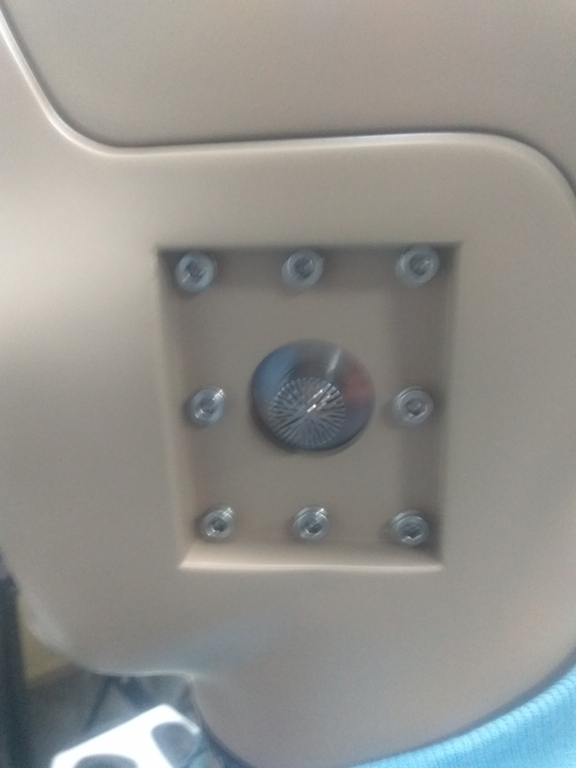
\includegraphics[width=0.25\linewidth]{day_0/ear}
				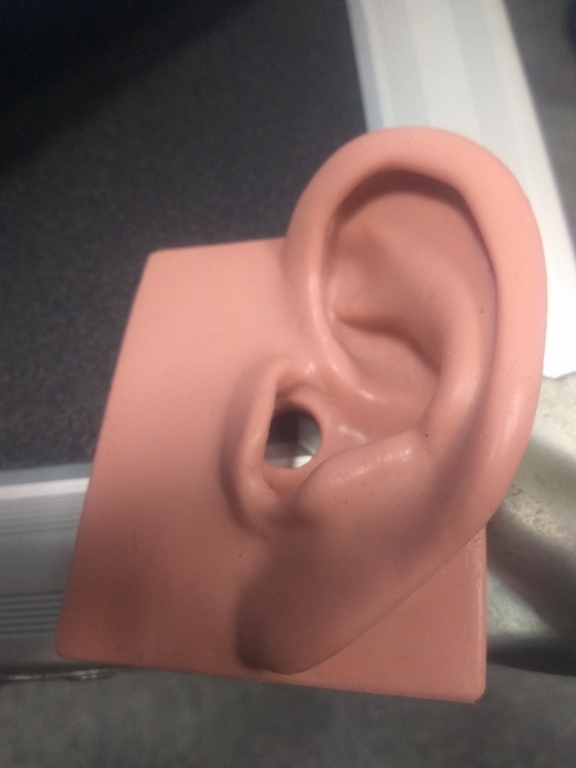
\includegraphics[width=0.25\linewidth]{day_0/earleaf}
			\end{figure}
		
			\newpage
			\item (\textit{kiri}) Konektor BNC, (\textit{tengah}) BNC output mic,  dan (\textit{kanan}) Audio DSP USB ke PC
			\begin{figure}[H]
				\centering
				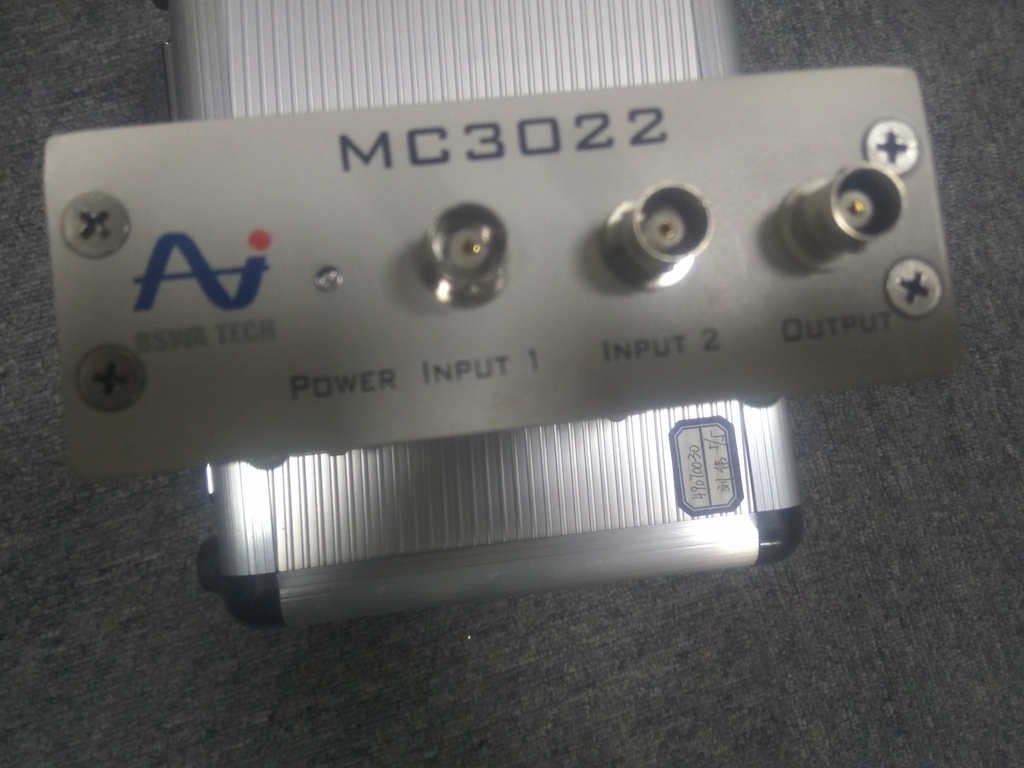
\includegraphics[width=0.25\linewidth]{day_0/bnc}
				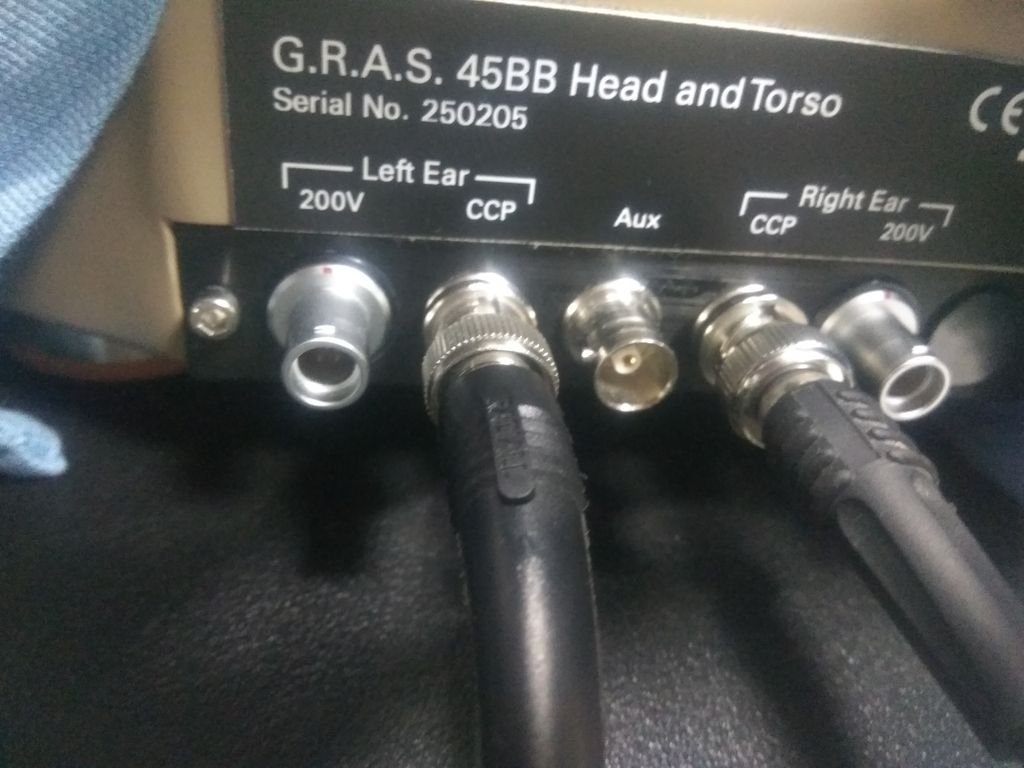
\includegraphics[width=0.25\linewidth]{day_0/bncout}
				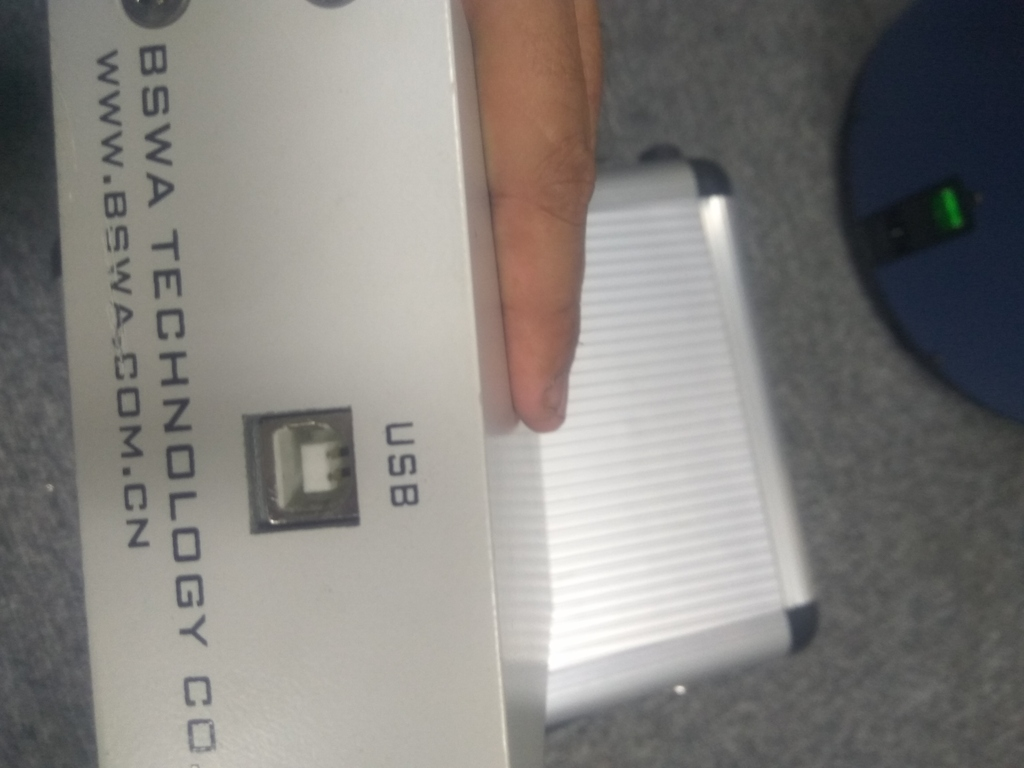
\includegraphics[width=0.25\linewidth]{day_0/usb}
			\end{figure}
		
			\item (\textit{kiri}) Unit Tone generator yg akan diuji dan (\textit{kanan}) setup pengujian
			\begin{figure}[H]
				\centering
				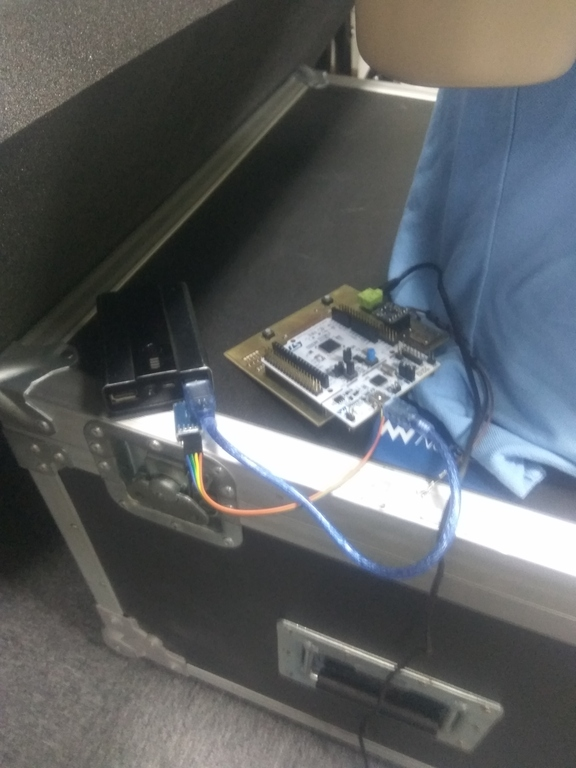
\includegraphics[width=0.25\linewidth]{day_0/testgen}
				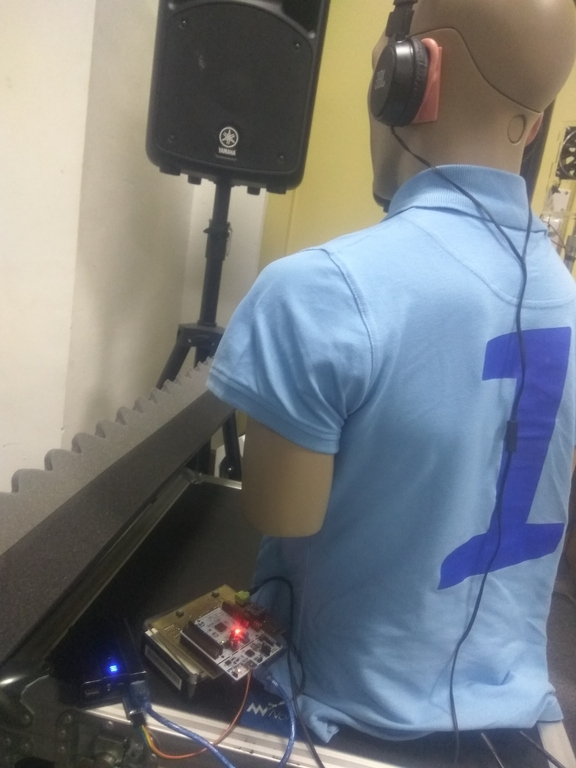
\includegraphics[width=0.25\linewidth]{day_0/setup}
			\end{figure}
		
			\item (\textit{kiri}) Audio DSP siap dan (\textit{kanan}) Contoh spectrogram respon
			\begin{figure}[H]
				\centering
				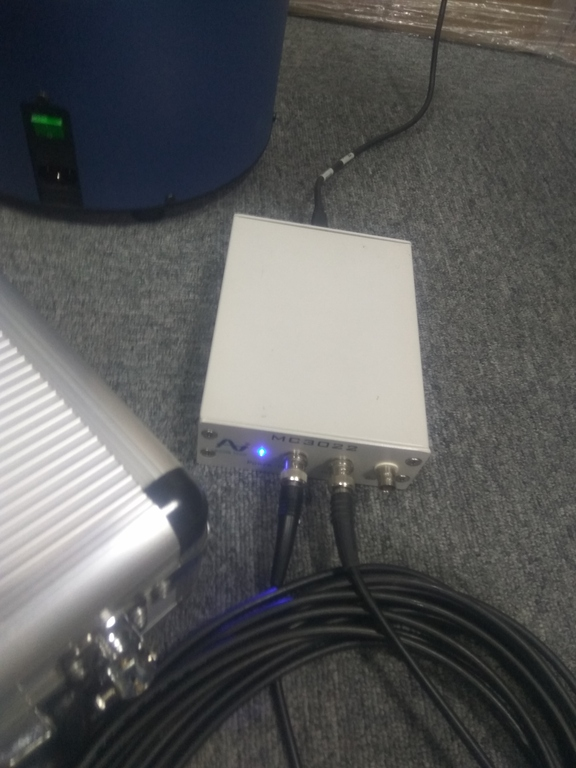
\includegraphics[width=0.25\linewidth]{day_0/runtest}
				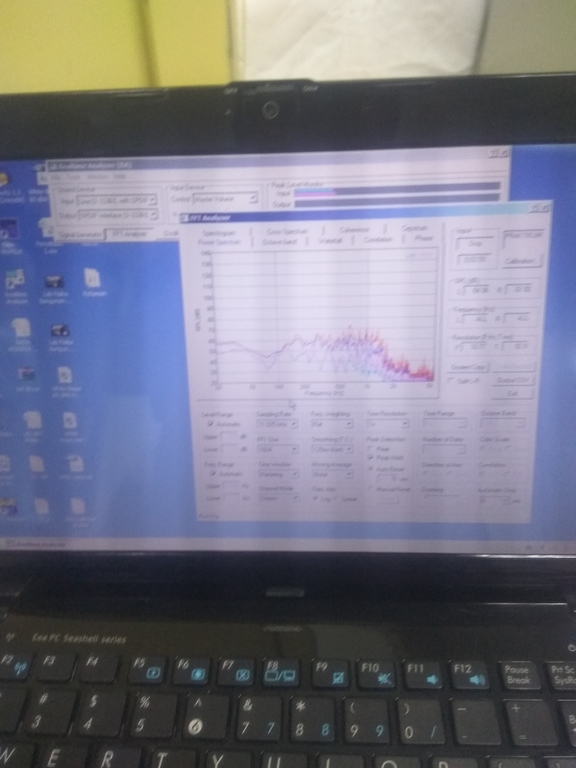
\includegraphics[width=0.25\linewidth]{day_0/test}
			\end{figure}
		
		\end{itemize}
	\end{itemize}	
	\subsubsection{Pengeluaran:}
	Tidak ada
	
	\subsection{13:00 - 14:00} 
	\subsubsection{Kegiatan:}
	\begin{itemize}
		\item Jalan kaki kembali ke Penginapan
		\item Istirahat di lobby penginapan
		\item Check-IN 
	\end{itemize}
	\subsubsection{Pengeluaran:}
	\begin{itemize}
		\item Gorengan
		\item Es Potong
		\item Air botolan
	\end{itemize}

	\subsection{14:00 - 16:30}
	\subsubsection{Kegiatan:}
	Tidur (pengganti insomnia di KA)
	
	\subsubsection{Pengeluaran:}
	Tidak ada
	
	\subsection{16:30 - 18:00}
	\subsubsection{Kegiatan:}
	Environment Look-Aroud. Jalan kaki sendirian menghafal detil lingkungan. Start at Daun Residence (Jln Juanda). End at Unikom Pusat (Jln Dipati-Ukur).
	Found:
	\begin{itemize}
		\item Bright-Mart (+ATM BNI)
		\item Circle K (+ATM BNI)
		\item ATM Centre (+ATM BNI)
		\item Unikom Cabang (+ATM BNI)
		\item Circle K
		\item Unikom Pusat (+ATM BNI) 
		\item Indomaret
		\item ATK+Fotokopi street
	\end{itemize}
	
	\subsubsection{Pengeluaran:}
	\begin{itemize}
		\item Gorengan
		\item T Connector
		\item Indomie 6
	\end{itemize}

	\subsection{18:00 - 20:00}
	\subsubsection{Kegiatan:}
	Nothing
	\subsubsection{Pengeluaran:}
	Air botolan
	
	\subsection{20:00 - 24:00}
	\subsubsection{Kegiatan}
	\begin{itemize}
		\item Komplain Wifi penginapan yang mati
		\item Rangkum log harian
		\item Draft rencana kegiatan esok
		\item Install Windows, Audacity, dan DSSF-3 di VBox
		\item Order Martabak (bukan ide saya) 
	\end{itemize}

	\subsubsection{Pengeluaran:}
	Martabak Telor
	
	\newpage
	\section{Day:2}
	
	\subsection{06:00 - 07:30}
	\subsubsection{Kegiatan:}
	\begin{itemize}
		\item Beli Notes kecil dan Pulpen
		\item Berangkat ke Lab Akustika
	\end{itemize}
	
	\subsubsection{Pengeluaran}
	\begin{itemize}
		\item Notes kecil
		\item Pulpen
		\item Kopi botolan
	\end{itemize}

	\subsection{08:00 - 13:00}
	\subsubsection{Kegiatan:}
	\begin{itemize}
		\item Setup KEMAR dan kebutuhan dasar
		\begin{itemize}
			\item Posisi Manekin dan Sudut Kepala di 0 derajat
			\begin{figure}[H]
				\centering
				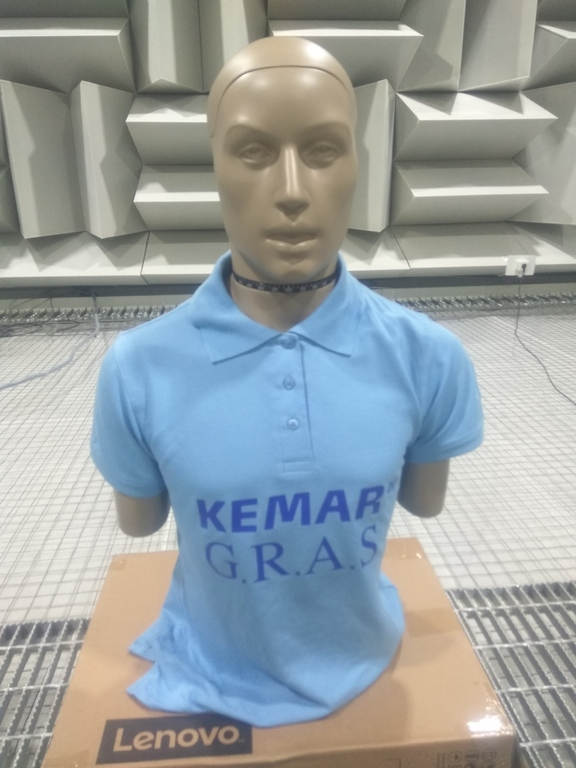
\includegraphics[width=0.25\linewidth]{day_1/manekin0}
				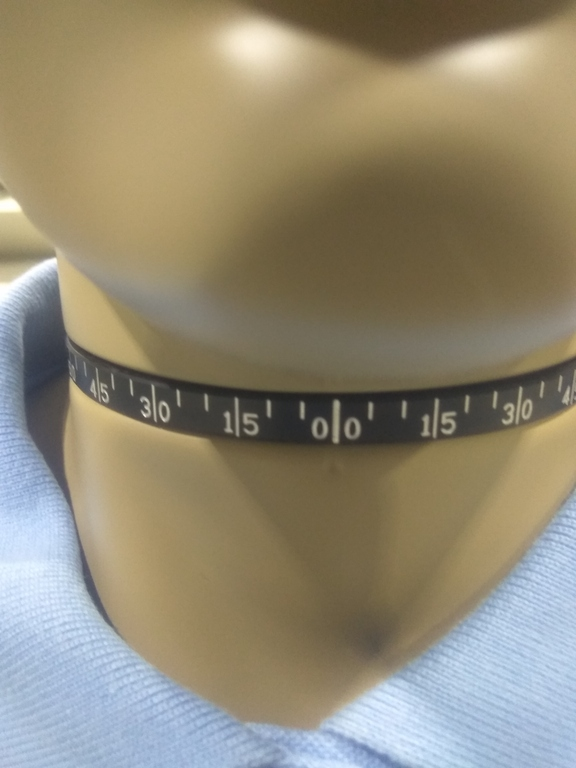
\includegraphics[width=0.25\linewidth]{day_1/manekin1}
				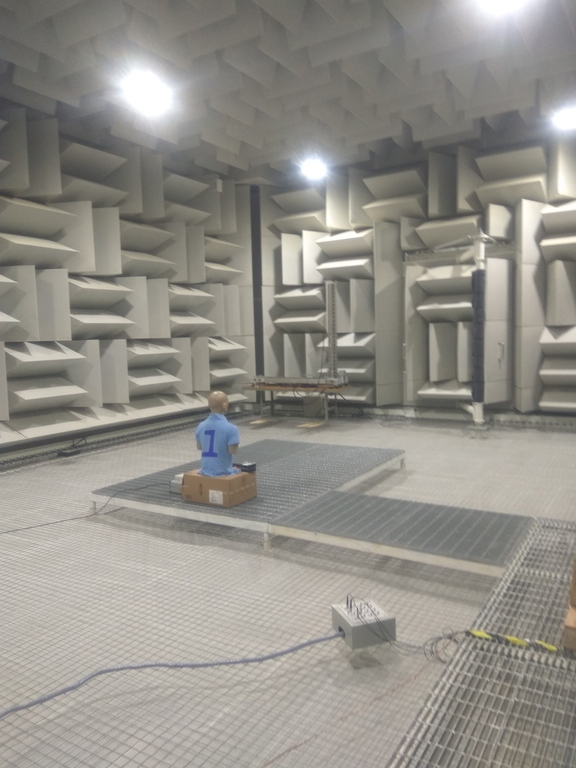
\includegraphics[width=0.25\linewidth]{day_1/manekin2}
			\end{figure}
			\item Pemasangan Daun Telinga Karet 
			\begin{figure}[H]
				\centering
				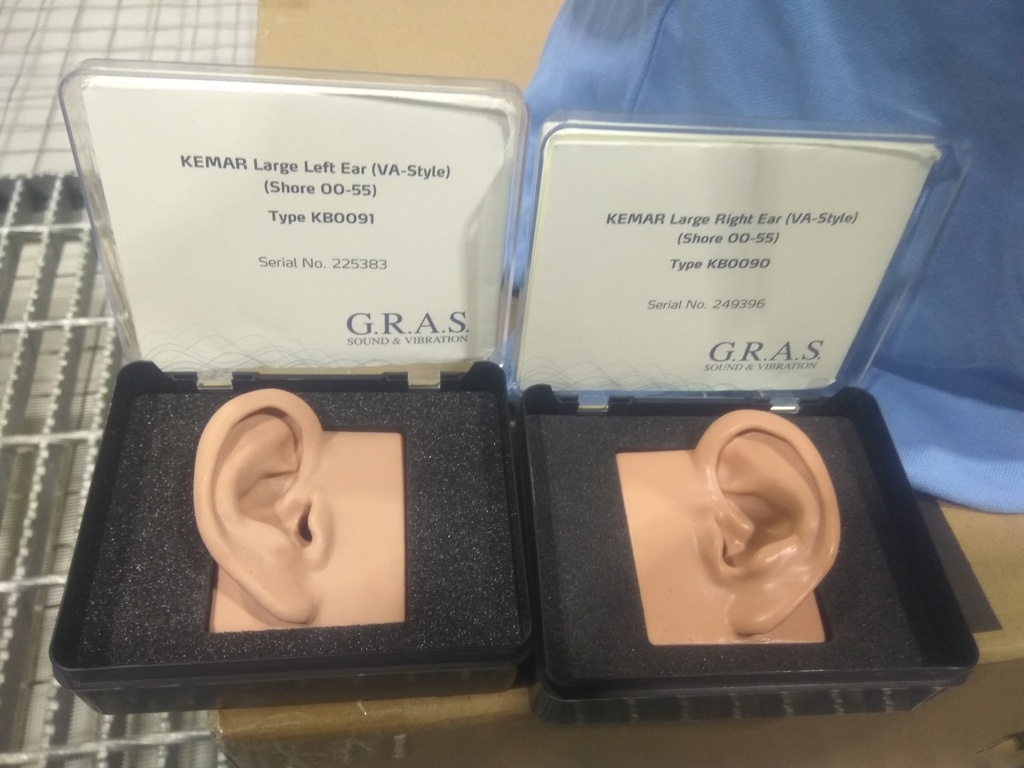
\includegraphics[width=0.25\linewidth]{day_1/earleaf0}
				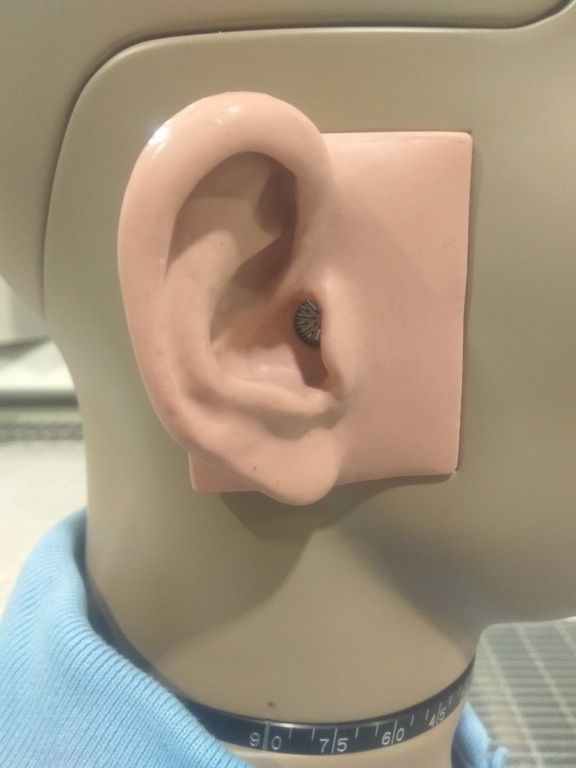
\includegraphics[width=0.25\linewidth]{day_1/earleaf1}
				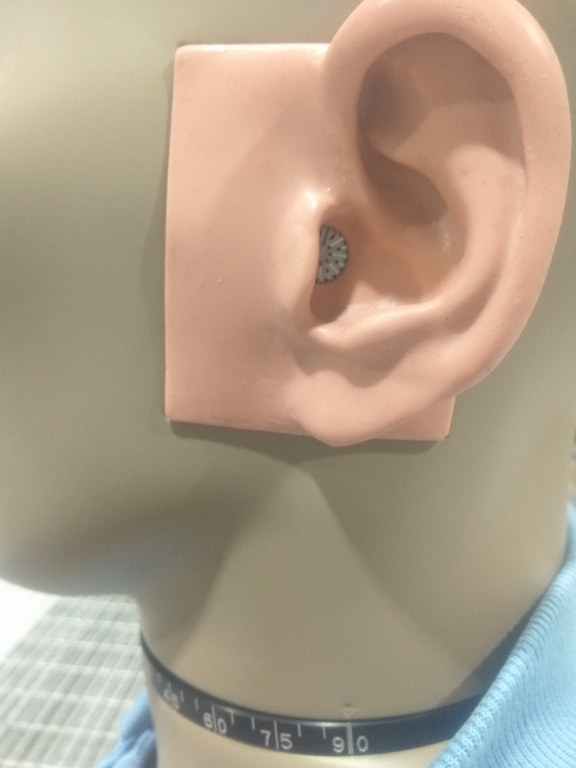
\includegraphics[width=0.25\linewidth]{day_1/earleaf2}
			\end{figure}
			\newpage
			\item Wiring Microphone Manekin ke Audio Card  
			\begin{figure}[H]
				\centering
				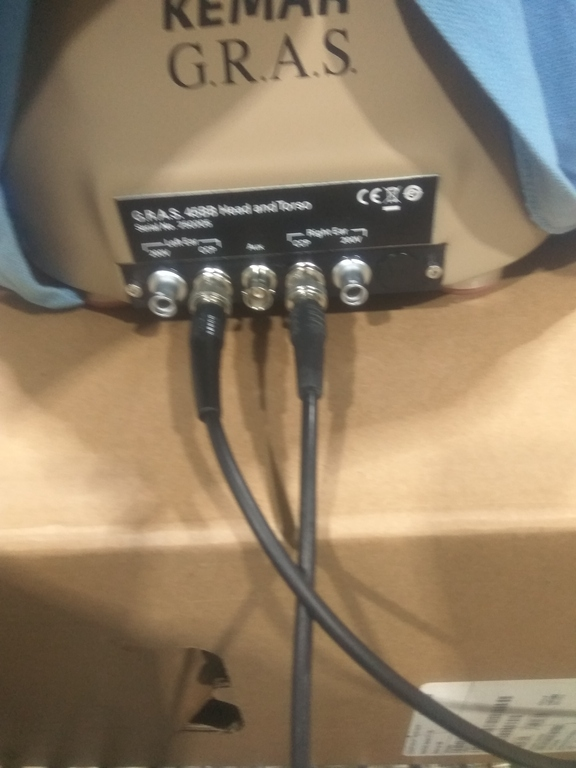
\includegraphics[width=0.25\linewidth]{day_1/wiring0}
				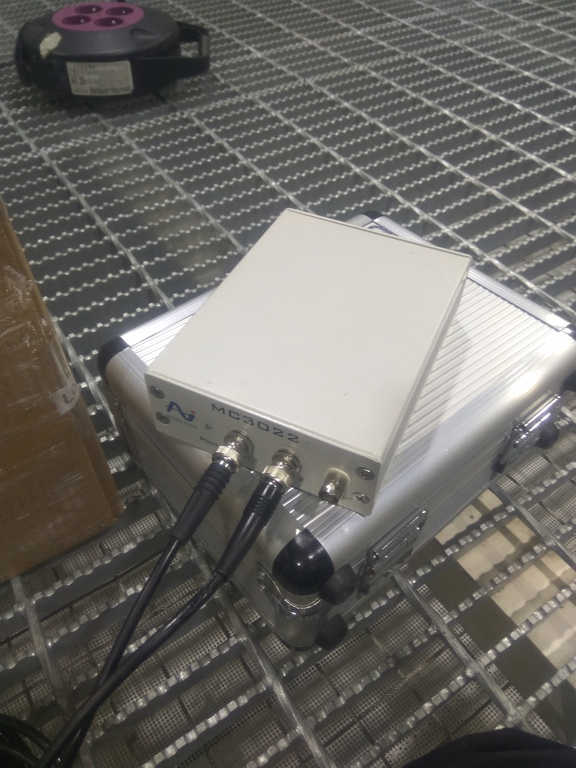
\includegraphics[width=0.25\linewidth]{day_1/wiring1}
			\end{figure}
			\item Kalibrasi Microphone KEMAR.
			Acuan standar uji kalibrasi ada di 114 dB dan 250 Hz.
			Kalibrasi di kedua microphone telinga.
			\begin{figure}[H]
				\centering
				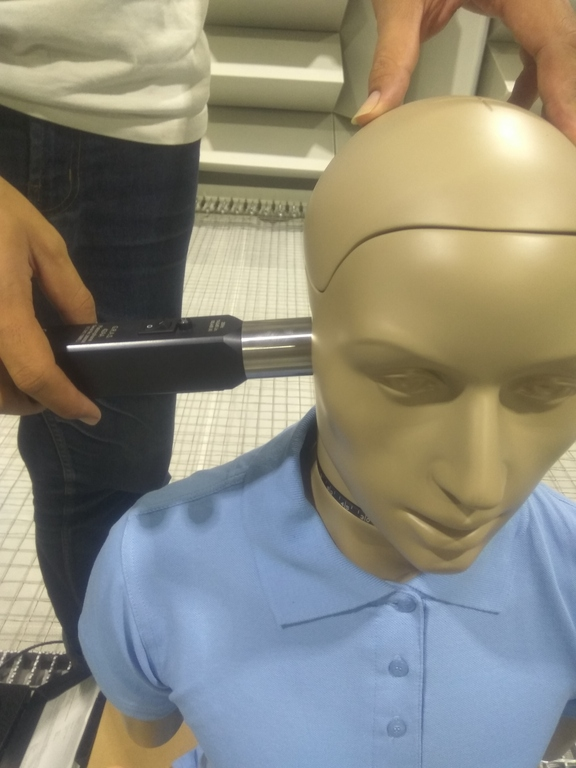
\includegraphics[width=0.25\linewidth]{day_1/kalib0}
				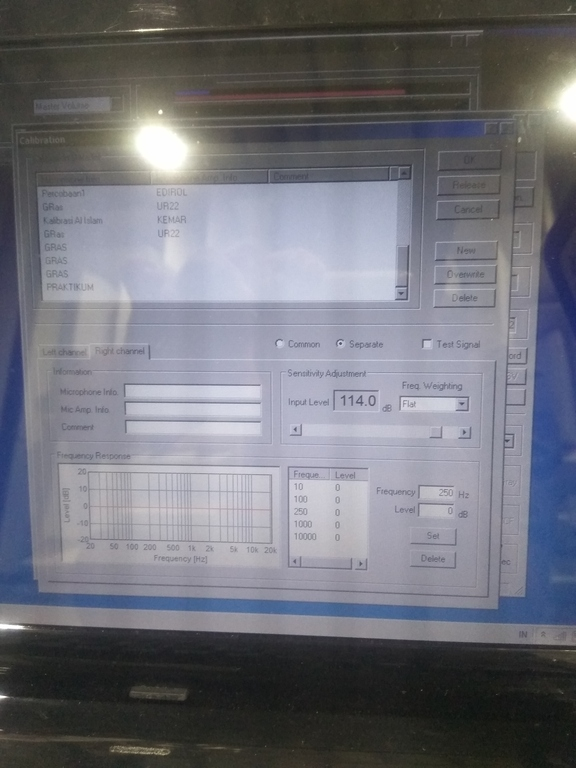
\includegraphics[width=0.25\linewidth]{day_1/kalib1}
				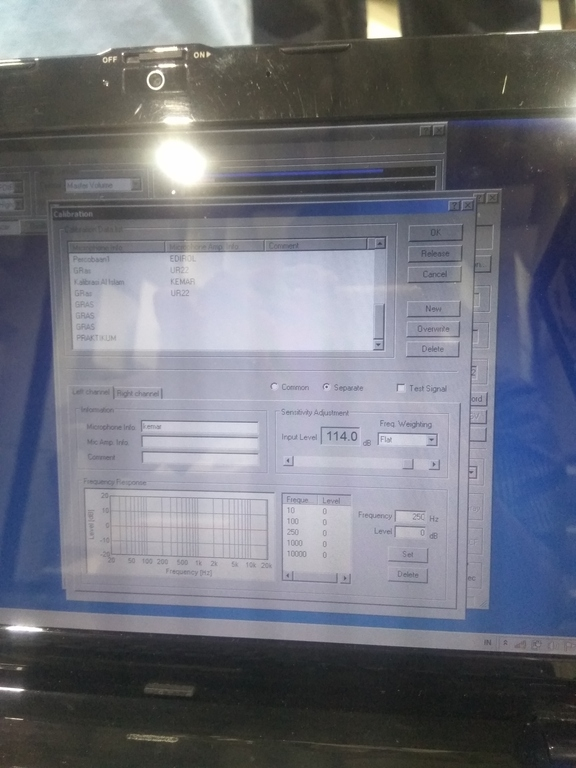
\includegraphics[width=0.25\linewidth]{day_1/kalib2}
			\end{figure}
			\item Pemasangan Headphone JBL.
			Cek speaker Headphone sudah menutupi lubang telinga atau belum.    
			\begin{figure}[H]
				\centering
				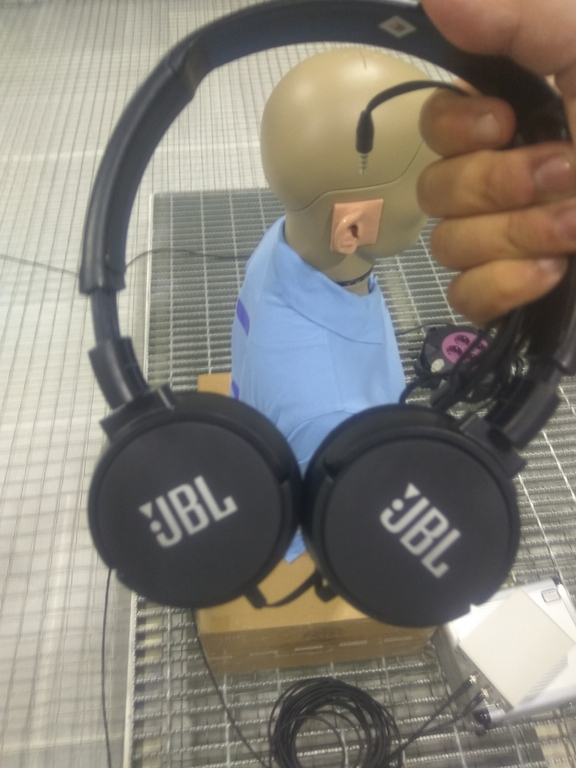
\includegraphics[width=0.25\linewidth]{day_1/phone0}
				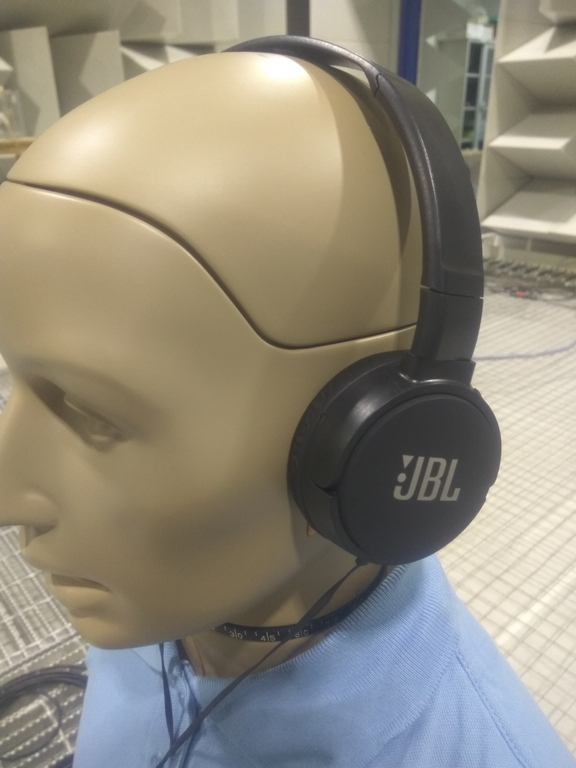
\includegraphics[width=0.25\linewidth]{day_1/phone1}
				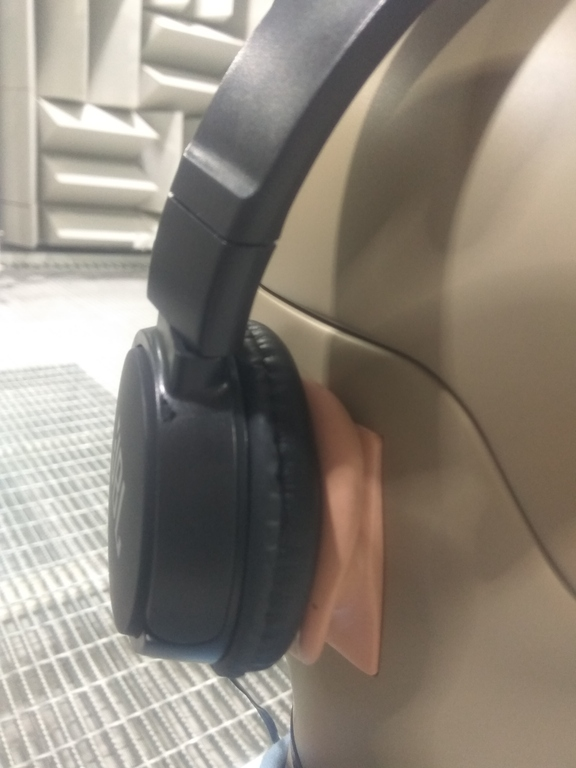
\includegraphics[width=0.25\linewidth]{day_1/phone2}
			\end{figure}
			\newpage
			
			\item Uji Flatness Frequency Response dari Headphone
			\begin{figure}[H]
				\centering
				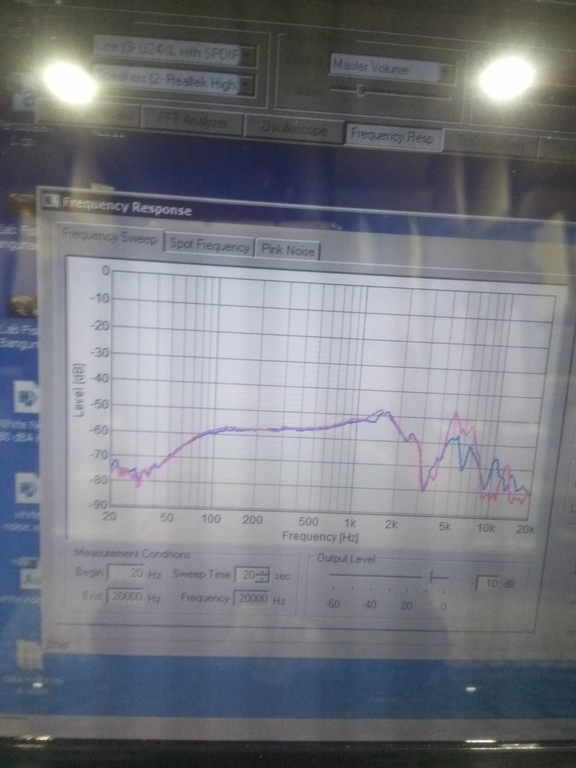
\includegraphics[width=0.25\linewidth]{day_1/resp0}
				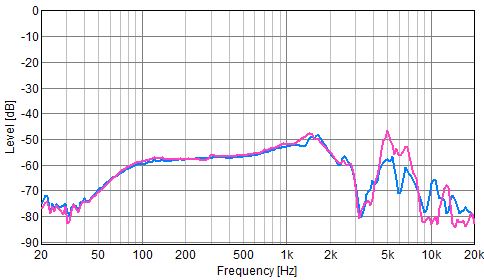
\includegraphics[width=0.5\linewidth]{day_1/resp1}
			\end{figure}
			
			\item Wiring Prototipe Wave-Generator yang akan diuji.
			Test awal menggunakan reversed-sine array.
			Protokol I2S di set pada Sampling Rate 16kHz pada clock 48MHz.
			Hasil ditampilkan di FFT Analyzer. 
			\begin{figure}[H]
				\centering
				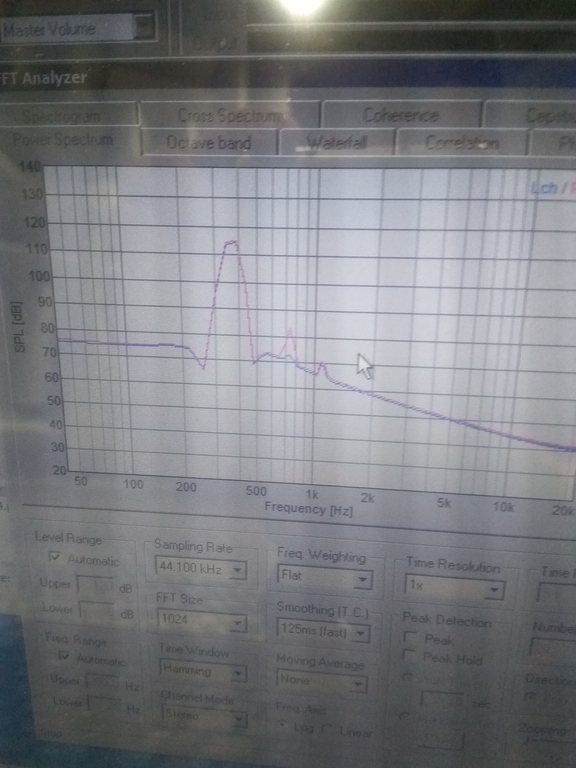
\includegraphics[width=0.25\linewidth]{day_1/test0}
				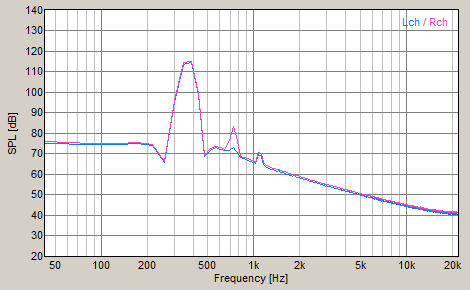
\includegraphics[width=0.5\linewidth]{day_1/test1}
			\end{figure}
			
			\item Setup siap
		\end{itemize}
		
		\item Uji Model Sine Wave array
		Berikut akan ditampilkan beberapa model Sine Wave array yang akan di feed ke PCM/I2S.
		Disertakan hasil FFT Analizer, pengaturan Clock I2S, Sampling Rate, dan ukuran buffer PCM.   
		
		\begin{itemize}
			\item Cek uji tanpa input (senyap) sebagai acuan dasar.
			Impedansi Audio DAC di set maximum (sesuai datasheet).
			\begin{figure}[H]
				\centering
				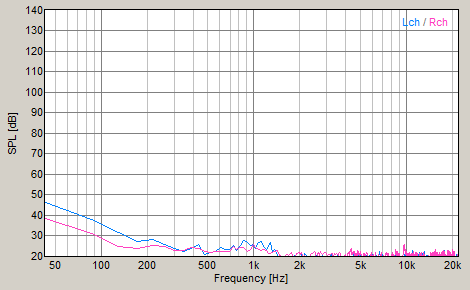
\includegraphics[width=0.5\linewidth]{result/BaseZero}
			\end{figure}
		
			\newpage
			\item Reversed-Sine Table.
			\begin{minted}[frame=lines,fontsize=\footnotesize]{c}
/*
 * Clk: 48MHz | SPR: 16kHz | Buff: 256
 */	
			\end{minted}
			\begin{figure}[H]
				\centering
				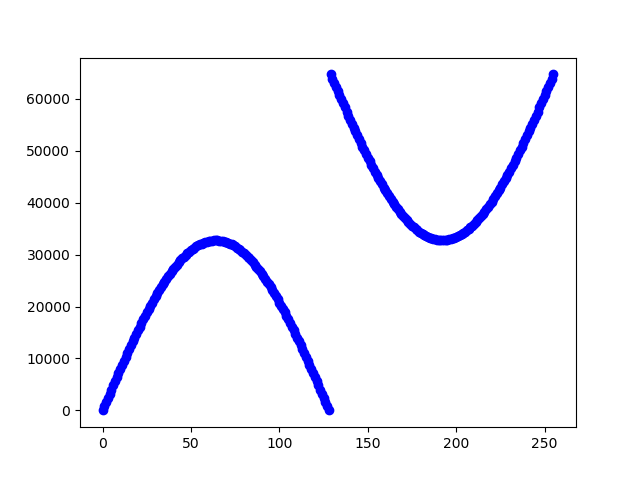
\includegraphics[width=0.45\linewidth]{result/rev_sine_table}
				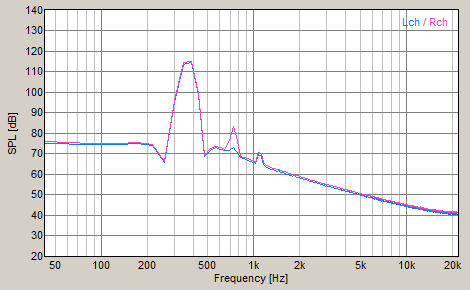
\includegraphics[width=0.45\linewidth]{result/tableMax256}
			\end{figure}
		
			\item Reversed-Sine loop formula.
			\begin{minted}[frame=lines,fontsize=\footnotesize]{c}
/*
* Clk: 48MHz | SPR: 16kHz | Buff: 256
*/
#define I2S_HALF_SIZE 127	
for(i=0;i<I2S_HALF_SIZE;i++){
	i2s_tx_buf[i] = 32767*sin(3.141592653589793*((double)i/(double)I2S_HALF_SIZE));
	i2s_tx_buf[I2S_HALF_SIZE+i] = 32767*(2-sin(3.141592653589793*((double)i/(double)I2S_HALF_SIZE)));
}
			\end{minted}
			\begin{figure}[H]
				\centering
				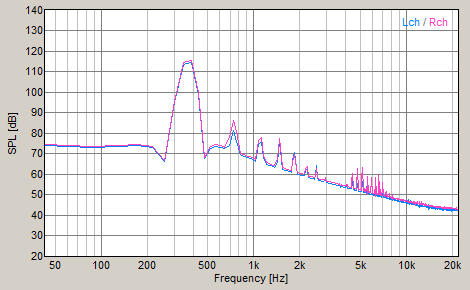
\includegraphics[width=0.5\linewidth]{result/halfMax256}
			\end{figure}
		
			\newpage
			\item Sine loop formula with buffer size 256.
			\begin{minted}[frame=lines,fontsize=\footnotesize]{c}
/*
* Clk: 48MHz | SPR: 16kHz | Buff: 256
*/
#define I2S_BUFF_SIZE 256	
for(i=0;i<I2S_BUFF_SIZE;i++){
	i2s_tx_buf[i] = 33767*sin((double) i*2*(M_PI/I2S_BUFF_SIZE));
}
			\end{minted}
			\begin{figure}[H]
				\centering
				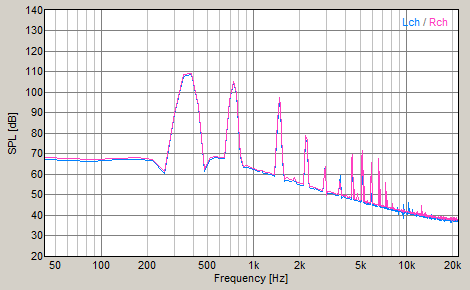
\includegraphics[width=0.5\linewidth]{result/max256}
			\end{figure}
		
			\item Sine loop formula with buffer size 512.
			\begin{minted}[frame=lines,fontsize=\footnotesize]{c}
/*
* Clk: 48MHz | SPR: 16kHz | Buff: 512
*/
#define I2S_BUFF_SIZE 512	
for(i=0;i<I2S_BUFF_SIZE;i++){
	i2s_tx_buf[i] = 33767*sin((double) i*2*(M_PI/I2S_BUFF_SIZE));
}
			\end{minted}
			\begin{figure}[H]
				\centering
				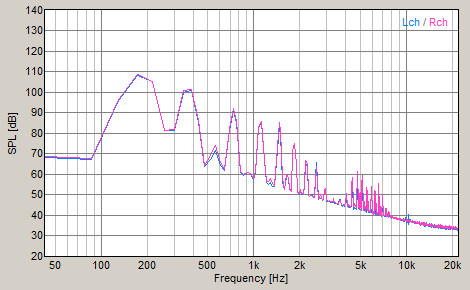
\includegraphics[width=0.5\linewidth]{result/max512}
			\end{figure}
		
			\newpage
			\item Sine loop formula with buffer size 1024.
			\begin{minted}[frame=lines,fontsize=\footnotesize]{c}
/*
* Clk: 48MHz | SPR: 16kHz | Buff: 1024
*/
#define I2S_BUFF_SIZE 1024	
for(i=0;i<I2S_BUFF_SIZE;i++){
	i2s_tx_buf[i] = 33767*sin((double) i*2*(M_PI/I2S_BUFF_SIZE));
}
			\end{minted}
			\begin{figure}[H]
				\centering
				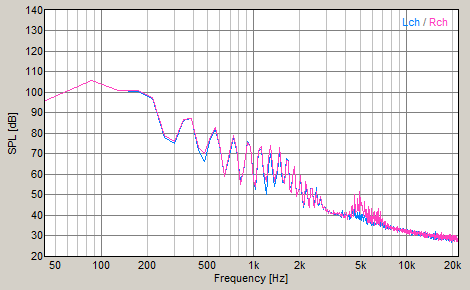
\includegraphics[width=0.5\linewidth]{result/max1024}
			\end{figure}
			
		\end{itemize}
	\end{itemize}
	
	\subsection{13:00 - 14:00}
	\subsubsection{Kegiatan:}
	Istirahat
	
	\subsubsection{Pengeluaran:}
	\begin{itemize}
		\item Gorengan
		\item Es teh botolan
	\end{itemize}

	\subsection{14:00 - 16:30}
	\subsubsection{Kegiatan:}
	\begin{itemize}
		\item Cek dan Uji untuk mendapatkan sebab derau di frekuensi yang yang lebih tinggi daripada frekuensi yang diingnkan.
		Hasilnya belum ketemu.
		\item Merapikan setup uji.
		\item Pulang kembali ke penginapan.
	\end{itemize}
	
	\subsubsection{Pengeluaran}
	Air Minum Botolan
	
	\newpage
	\subsection{17:00 - 20:00}
	\subsubsection{Kegiatan:}
	\begin{itemize}
		\item Istirahat/Tidur.
		\item Refreshing 
	\end{itemize}

	\subsubsection{Pengeluaran:}
	\begin{itemize}
		\item Kopi Botolan
		\item Sang Pisang (bukan ide saya)
	\end{itemize}

	\subsection{20:00 - 02:00}
	Mempelajari semua dokumentasi Protokol PCM/I2S, Audio DAC MAX98375A, dan implementasinya HAL ChibiOS/RT untuk STM32. 
	
	\newpage
	\section{Day:3}
	\subsection{07:00 - 14:00}
	\subsubsection{Kegiatan:}
	\begin{itemize}
		\item Berangkat ke lab dan melanjutkan uji model Sine Wave array
		Semua hasil pengujian hari ini menggunakan pengaturan baru di chip, yaitu:
		(1) Linking Time Optimization (LTO) dari GCC diaktifkan dan
		(2) Floating-Point Unit (FPU) menggunakan internal Cortex-M4.
		
		Berikut hasil sementara:
		\begin{itemize}
			\item Reversed-Sine loop formula skala satu.
			\begin{minted}[frame=lines,fontsize=\footnotesize]{c}
/*
* Clk: 48MHz | SPR: 16kHz | Buff: 256 | Scale: 1
*/
#define I2S_HALF_SIZE 127	
for(i=0;i<I2S_HALF_SIZE;i++){
	i2s_tx_buf[i] = 32767*sin(3.141592653589793*((double)i/(double)I2S_HALF_SIZE));
	i2s_tx_buf[I2S_HALF_SIZE+i] = 32767*(2-sin(3.141592653589793*((double)i/(double)I2S_HALF_SIZE)));
}
			\end{minted}
			\begin{figure}[H]
				\centering
				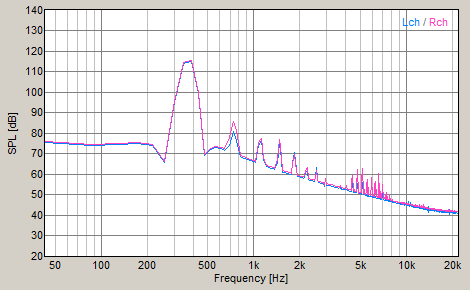
\includegraphics[width=0.5\linewidth]{result/tone1}
			\end{figure}
		
			\item Reversed-Sine loop formula skala setengah.
			\begin{minted}[frame=lines,fontsize=\footnotesize]{c}
/*
* Clk: 48MHz | SPR: 16kHz | Buff: 256 | Scale: 0.5
*/
#define I2S_HALF_SIZE 127	
for(i=0;i<I2S_HALF_SIZE;i++){
	i2s_tx_buf[i] = 32767*sin(3.141592653589793*((double)i/(double)I2S_HALF_SIZE));
	i2s_tx_buf[I2S_HALF_SIZE+i] = 32767*(2-sin(3.141592653589793*((double)i/(double)I2S_HALF_SIZE)));
}
			\end{minted}
			\begin{figure}[H]
				\centering
				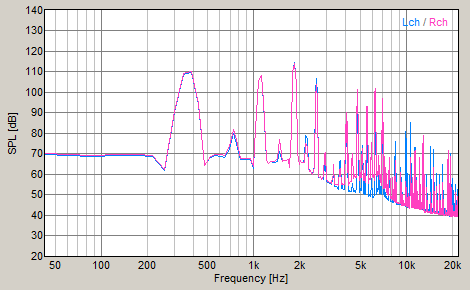
\includegraphics[width=0.5\linewidth]{result/tone05}
			\end{figure}
		
			\newpage
			\item Sine loop formula pada Clock I2S 48MHz.
			\begin{minted}[frame=lines,fontsize=\footnotesize]{c}
/*
* Clk: 48MHz | SPR: 16kHz | Buff: 256
*/
#define STM32_PLLI2SN_VALUE 288
#define STM32_PLLI2SR_VALUE 6
#define I2S_BUFF_SIZE 256	
for(i=0;i<I2S_BUFF_SIZE;i++){
	i2s_tx_buf[i] = 33767*sin((double) i*2*(M_PI/I2S_BUFF_SIZE));
}
			\end{minted}
			\begin{figure}[H]
				\centering
				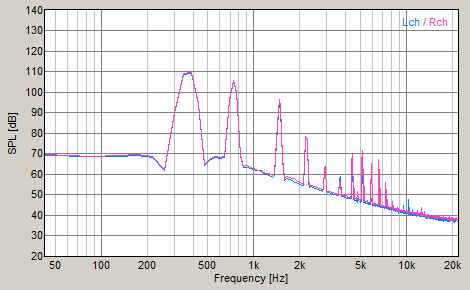
\includegraphics[width=0.5\linewidth]{result/sine_clk48}
			\end{figure}
		
			\item Sine loop formula pada Clock I2S 72MHz.
			\begin{minted}[frame=lines,fontsize=\footnotesize]{c}
/*
* Clk: 72MHz | SPR: 16kHz | Buff: 256
*/
#define STM32_PLLI2SN_VALUE 288
#define STM32_PLLI2SR_VALUE 6
#define I2S_BUFF_SIZE 256	
for(i=0;i<I2S_BUFF_SIZE;i++){
	i2s_tx_buf[i] = 33767*sin((double) i*2*(M_PI/I2S_BUFF_SIZE));
}
			\end{minted}
			\begin{figure}[H]
				\centering
				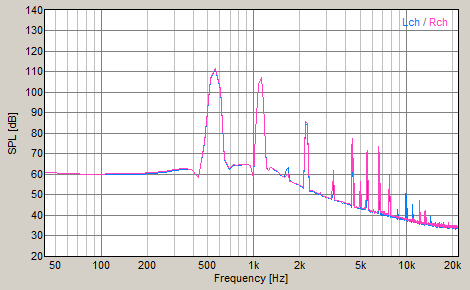
\includegraphics[width=0.5\linewidth]{result/sine_clk72}
			\end{figure}
			
			\newpage
			\item Sine loop formula pada Clock I2S 96MHz.
			\begin{minted}[frame=lines,fontsize=\footnotesize]{c}
/*
* Clk: 96MHz | SPR: 16kHz | Buff: 256
*/
#define STM32_PLLI2SN_VALUE 288
#define STM32_PLLI2SR_VALUE 3
#define I2S_BUFF_SIZE 256	
for(i=0;i<I2S_BUFF_SIZE;i++){
	i2s_tx_buf[i] = 33767*sin((double) i*2*(M_PI/I2S_BUFF_SIZE));
}
			\end{minted}
			\begin{figure}[H]
				\centering
				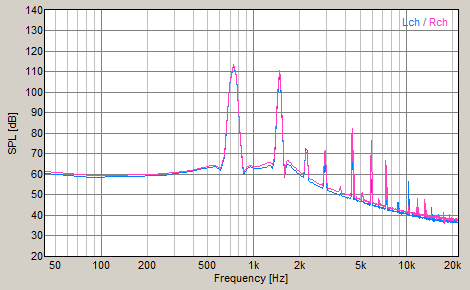
\includegraphics[width=0.5\linewidth]{result/sine_clk96}
			\end{figure}
		
			\item Sine loop formula pada ukuran array size 44100.
			\begin{minted}[frame=lines,fontsize=\footnotesize]{c}
/*
* Clk: 96MHz | SPR: 16kHz | Buff: 256 | Array: 44100
*/
#define STM32_PLLI2SN_VALUE 288
#define STM32_PLLI2SR_VALUE 3
#define I2S_BUFF_SIZE 256	
uint16_t i2s_tx_buf[44100];
for(i=0;i<I2S_BUFF_SIZE;i++){
	i2s_tx_buf[i] = 33767*sin((double) i*2*(M_PI/I2S_BUFF_SIZE));
}
			\end{minted}
			\begin{figure}[H]
				\centering
				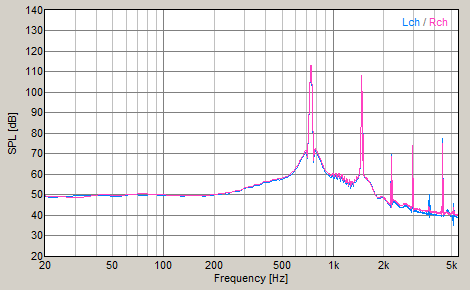
\includegraphics[width=0.5\linewidth]{result/arr_spr_sine}
			\end{figure}
		
			\newpage
			\item Reversed-Sine loop formula pada ukuran array size 44100.\\
			Hingga laporan ini dibuat, Model sine ini adalah yang paling baik 
			dan mudah dimodifikasi amplitudo tanpa menggeser frekuensi
			serta paling sedikit noise di frekuensi di atas frekuensi yang diinginkan. 
			\begin{minted}[frame=lines,fontsize=\footnotesize]{c}
/*
* Clk: 96MHz | SPR: 16kHz | Buff: 256 | Array: 44100
*/
#define STM32_PLLI2SN_VALUE 288
#define STM32_PLLI2SR_VALUE 3
#define I2S_HALF_SIZE 127	
uint16_t i2s_tx_buf[44100];
double ampl;
for(i=0;i<I2S_HALF_SIZE;i++){
	i2s_tx_buf[i] = 32767*ampl*sin(3.141592653589793*((double)i/(double)I2S_HALF_SIZE));
	i2s_tx_buf[I2S_HALF_SIZE+i] = 32767*(2-ampl*sin(3.141592653589793*((double)i/(double)I2S_HALF_SIZE)));
}
			\end{minted}
			\begin{figure}[H]
				\centering
				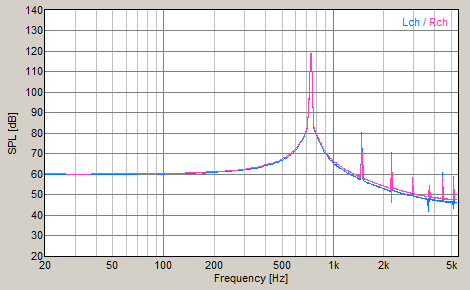
\includegraphics[width=0.5\linewidth]{result/arr_spr_revsine}
			\end{figure}
		
			Untuk konfirmasi dari mana asal derau di frekuensi lebih tinggi dari frekuensi yang diinginkan,
			maka digunakan osiloskop digital dengan analog frekuensi sampling di 200kHz.
			\begin{figure}[H]
				\centering
				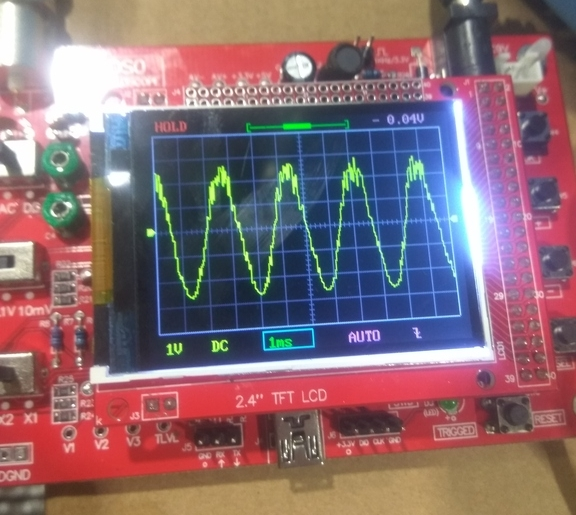
\includegraphics[width=0.5\linewidth]{result/osiloskop}
			\end{figure}
			
			Dugaan awal, model array yang dikirim ke PCM/I2S ditumpangkan ke sinyal dasar sinus frekuensi tinggi,
			dimana sinyal ini tidak benar-benar hilang pada output akhir.
		\end{itemize}
	\end{itemize}

	\newpage
	\subsection{14:00 - 18:00}
	\subsubsection{Kegiatan:}
	\begin{itemize}
		\item Pulang
		\item Istirahat/Tidur
		\item Refreshing
	\end{itemize}
	\subsubsection{Pengeluaran}
	\begin{itemize}
		\item Sarapan Nasi Ikan
		\item Air botol dingin
	\end{itemize}

	\subsection{18:00 - 23:00}
	\subsubsection{Kegiatan:}
	\begin{itemize}
		\item Review catatan kegiatan.
		\item Buat Log Kegiatan Harian dan Hasil Pengujian sementara.
		\item Pengujian dengan bantuan osiloskop:
		\begin{itemize}
			\item Array size turun dari 44100 ke 16000.
			Menyesuaikan I2S Sampling Rate
			\item Menggunakan Murni DC power supply.
			Power Bank 5v/2A.
			Untuk menguji efek PSRR (Power Supply Reject Ratio).
		\end{itemize}
		Hasil keduanya tidak berbeda signifikan.
		\begin{figure}[H]
			\centering
			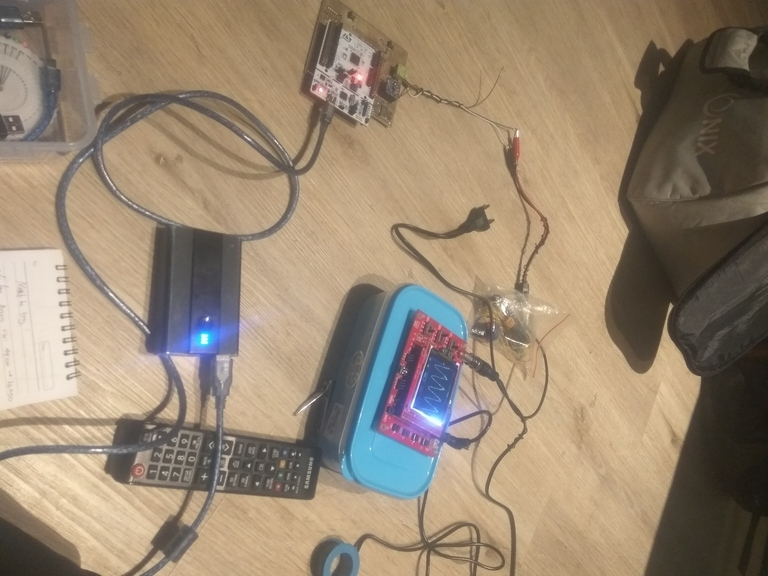
\includegraphics[width=0.5\linewidth]{result/nighttest}
		\end{figure}
		\item Menambahkan fitur shutdown DAC untuk set ke impedance maximal saat tidak ada output.
		\item Istirahat/Tidur.
	\end{itemize}
	
\end{document}